\documentclass[11pt,a4paper]{article}

\usepackage[T1]{fontenc}
\usepackage[utf8]{inputenc}
\usepackage[frenchb]{babel}

\usepackage{fancyhdr} % headers
\usepackage[usenames,dvipsnames]{color} % colors
\usepackage{graphicx} % images
\usepackage{listings} % source code
\usepackage{titling} % meta-infos
\usepackage{courier} % courier font
\usepackage{fullpage} % full page layout
\usepackage{titlesec} % title customization
\usepackage{parskip} % paragraphs spacing
\usepackage{amsmath}
\usepackage{tikz}
\usepackage{siunitx}
%\usepackage{showframe} % layout debug

\usepackage{float}
%\floatstyle{boxed}
\restylefloat{figure}
\usepackage[nottoc,numbib]{tocbibind}

\topmargin -10mm
\headsep 5mm
\headheight 10mm

\linespread{1.0}
\renewcommand{\arraystretch}{1.3}

%\setlength\parindent{0pt}
\setlength{\unitlength}{1cm}
\setlength{\droptitle}{-1.6cm}

\pagestyle{fancy}
\fancyhf{}
\cfoot{\thepage}

\def \doccourse { INF2-B -- Présentation }
\def \doctitle {Gestion de versions avec Git}
\author{Bastien Clément \and Christophe Peretti}

%\renewcommand{\thesection}{Objectif \arabic{section} :}
%\renewcommand{\thesubsection}{\arabic{section}.\arabic{subsection}}

\rhead{\theauthor \\ \today}
\lhead{\doccourse \\ \doctitle }
\title{{\normalsize \doccourse} \\ \doctitle }

\setlength{\droptitle}{3cm}

\begin{document}
\pagenumbering{gobble}

\maketitle

\vspace{4cm}
\begin{center}

\includegraphics[width=5cm]{git_logo}
\end{center}

\pagebreak

\tableofcontents

\pagebreak
\pagenumbering{arabic}

\section{Introduction à la gestion de versions}

\textit{Git} est un logiciel de gestion de versions libre et open-source.
Avant de s'y attaquer directement, il est nécessaire de commencer par une petite introduction sur le concept de gestion de version.
De quoi s'agit-il et pourquoi est-ce intéressant dans le domaine de la programmation logiciel ?

Dans son modèle le plus simple, un logiciel de gestion de versions est chargé d'enregistrer les modifications apportées à un ensemble de fichier au cours du temps.
Par la suite, il est possible de naviguer dans cet historique pour consulter ou récupérer d'anciennes versions d'un fichier spécifique.
Dans notre cas, nous l'utiliserons typiquement pour conserver l'historique du code source de nos programmes.

\subsection{Gestion de version locale}

Une façon de mettre en place un système de gestion de versions très simpliste serait d'effectuer périodiquement des copies du dossier du projet en les annotant avec la date et l'heure de la copie.
Il est alors possible de retourner dans une copie particulière pour avoir accès à une version antérieur d'un fichier.
Des logiciels automatiques sur le même principe sont même intégrés directement aux système d'exploitation comme par exemple \textit{Time Machine} sur \textit{OS X} et \textit{File History} sur \textit{Windows}.
Les sauvegardes sont cependant effectuées automatiquement à intervalles régulières et ne correspondent pas aux étapes du développement du logiciel.

Les logiciels spécialisés (tel que \textit{rcs}, développé depuis 1982) permettent à l'inverse d'effectuer des sauvegardes à des moments particuliers, typiquement lorsqu'une fonctionnalité du programme est terminée et prête à être sauvegardée.
Ces logiciels fournissent ainsi un niveau de \textit{sécurité} et d'\textit{historique}, constituant les premières facettes de la gestion de versions.

\subsection{Gestion de version centralisée}

Une autre facette de la gestion de versions est la \textit{collaboration}. 

Le développement de logiciels, pour tout projet un minimum sérieux, implique généralement la collaboration de plusieurs développeurs.
Même dans le cadre de nos laboratoires encore relativement simples, nous avons pu constater les difficultés liées au développement à plusieurs.
Comment rester à jour sur le travail effectué par notre binôme ?
Comment garder une copie cohérente du projet lorsqu'un fichier est modifiés par plus d'une personne au même moment ?

Les logiciels de gestion de versions centralisés règlent ce problème en se basant sur un \textit{dépôt} central dans lequel les fichiers constituant la version de référence du logiciel sont enregistrés.
C'est le cas par exemple du logiciel \textit{Subversion} (souvent abrégé \textit{svn}).

\begin{figure}[H]
\begin{center}
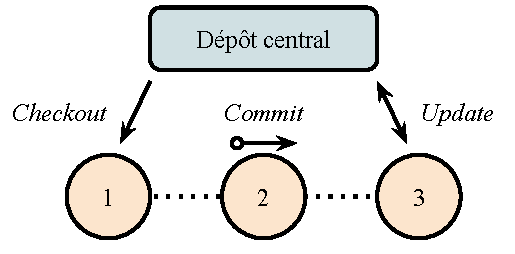
\includegraphics[width=7cm]{img_cvcs} \\
\caption{\small \textit{Workflow} typique d'un système de gestion de versions centralisé}
\end{center}
\end{figure}

Lorsqu'un développeur souhaite modifier le logiciel, il commence par en effectuer une copie sur sa machine (opération \textit{checkout}), modifie et enregistre son travail localement (opération \textit{commit}), puis il termine en envoyant ses modifications sur le dépôt central (opération \textit{update}) pour qu'elles soient intégrées définitivement au logiciel.
Il récupère au passage les modifications des autres développeurs et est informés des situations de conflits, c'est à dire deux modifications différentes sur la même partie de code, qu'il doit résoudre avant de pouvoir continuer.

En revanche, dans cette configuration, le dépôt central constitue un \textit{single point of failure}.
S'il est inaccessible, la collaboration et l'envoi des modifications deviennent temporairement impossible.
Si un problème plus grave survient, en l'absence de sauvegarde récente, une partie ou l'ensemble de l'historique du projet peut être définitivement perdu ou corrompu.

\subsection{Gestion de version distribuée}

À l'inverse, dans un système décentralisé tel que Git (mais aussi \textit{Mercurial} ou \textit{Bazaar}), lorsqu'une copie locale du projet est effectuée, ce n'est pas uniquement les dernières versions des fichiers qui sont récupérées, mais l'ensemble de l'historique du dépôt.
On parle alors de \textit{clônage}.

Il n'y a ainsi plus de dépôt central à proprement parler et chaque développeur possède naturellement un copie complète de l'historique du projet. Puisque toutes les informations sont disponibles localement, la majorités des opérations peuvent être effectuées hors-ligne et sont ainsi beaucoup plus rapides.

%En l'absence de dépôt central, l'utilisateur est libre de choisir la méthode d'échange des modifications avec ses collaborateurs qui se résume à transmettre un fichier contenant l'ensembles des modifications apportées entre deux versions du projet.
%Les autres développeurs pourront alors fusionner ces changements dans leur copie locale.

Bien entendu, l'utilisation d'un dépôt centralisé simplifie grandement la collaboration et permet d'avoir une version de référence accessible à tous en permanence.
Git supporte la notion de dépôt distant (\textit{remote}) depuis lesquels il peut récupérer ou envoyer des modifications.

\begin{figure}[H]
\begin{center}
\vspace{1em}
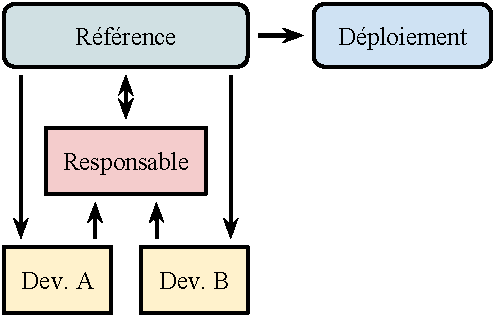
\includegraphics[width=7.5cm]{img_dvcs} \\
\caption{\small Exemple d'organisation à plusieurs niveaux}
\end{center}
\end{figure}

Dans l'exemple ci-dessus, les développeurs clônent le dépôt de référence et effectue leurs modifications.
Ils transmettent ensuite ces modifications au responsable du projet qui se chargera de les valider et de les intégrer au code de référence.
Par la suite, lorsque une nouvelle version du projet est prête à être distribuée, le dépôt est copié dans un dépôt particulier sur un serveur de déploiement.
Cette opération déclenchera par exemple la compilation et distribution automatique du logiciel mis à jour.
On peut noter que dans cette configuration, un simple développeur ne peut jamais modifier la version de référence sans passer par le responsable du projet.

Puisqu'il n'y a plus nécessairement de dépôt central unique, il est possible d'organiser le développement de façon très flexible en fonction de ce qui est le plus adapté à chaque situation.

%Ainsi, il suffit d'utiliser un simple clône sur un serveur pour reproduire le modèle de collaboration des logiciels centralisés sans les problèmes de disponibilités puisqu'il est toujours possible de transmettre ses changements par d'autres canaux.
%En pratique, c'est le modèle d'utilisation de \textit{Git} le plus courant aujourd'hui.

\pagebreak
\section{Git}

\subsection{Histoire}

Les origines de Git sont étroitement liées à l'organisation du développement du noyau Linux, développés tout deux par Linus Torvalds.

Dans un premier temps, de 1991 à 2002, les développeurs et contributeurs de Linux n'utilisaient pas de logiciels particuliers et échangeaient leur travail sous forme de \textit{patches} et d'archives.
Face aux difficultés engendrées par la croissance du projet, la décision d'utiliser le logiciel de gestion de versions propriétaire BitKeeper est prise.
L'éditeur proposait alors une licence gratuite permettant, sous certaines conditions, d'utiliser avec quelques limitations le programme gratuitement pour le développement de logiciels libre.

En 2005, un conflit entre un développeur indépendant de l'organisation OSDL (\textit{Open Source Development Labs}) et la société éditrice BitMover conduit à la résiliation de la licence spécifique pour les logiciels libres.
Bien que BitMover propose de continuer à fournir gratuitement son logiciel à certains développeurs de Linux, elle le refuse à Linus Torvalds, également membre de l'OSDL.
L'utilisation controversée de BitKeeper est alors abandonnée et le projet Git est lancé avec pour but de devenir le logiciel de gestion de versions utilisés par tous les développeurs du noyau Linux.

\subsection{Installation}

Git peut être téléchargé gratuitement depuis le site officiel du projet {\tt http://git-scm.com/}.

Le logiciel est disponible sur tous les systèmes d'exploitation principaux.
La version pour Windows intègre également une extensions pour l'explorateur de fichiers permettant d'accéder aux commandes de Git en utilisant les menus contextuels.

\subsection{Branchement et fusion}

\subsubsection{Conflits}

\subsection{Distribué}

\subsection{Intégrité des données}

\subsection{\textit{Staging area}}

\pagebreak
\section{Organisation du développement avec branches}

\subsection{Structure d'un \textit{commit}}

\subsection{Branches}

\subsection{Fusion}

\subsection{Conflits}

\pagebreak
\section{GitHub}

GitHub est un site internet d'hébergement et de gestion de développement de logiciels basé sur Git.
Il a été lancé le 10 avril 2008, soit 2 ans seulement après le projet Git lui-même et a joué un rôle important dans son adoption rapide par les développeurs.
La plateforme est aujourd'hui un site incontournable dans le monde du logiciel open-source, utilisé même par de grands noms tel que Google et Microsoft. 

\subsection{Modèle \textit{Fork / Pull Requests}}


\subsection{Offre pour les étudiants}

L'hébergement de dépôt sur GitHub est entièrement gratuit pour les projets open-source. En revanche, il est nécessaire souscrire à un abonnement pour pouvoir réer des dépôts privés dont l'accès est limité aux personnes autorisées.

Heusement, GitHub propose aux personnes possédant une adresse e-mail provenant d'une université reconnue (tel que la HEIG-VD!) un plan \textit{Micro} gratuit pendant toute la durée des études, soit 5 dépôts privés avec un nombre illimités de collaborateurs par dépôt.

L'inscription se fait à l'adresse {\tt https://education.github.com/} et est accompagnée d'autres offres pour former le {\it Student Developer Pack}.

\section{Conclusion}

-> Learning curve

\pagebreak
\pagenumbering{roman}

\begin{thebibliography}{1}

\bibitem{progit}
	CHACON, Scott et STRAUB, Ben. {\em Pro Git} (2e éd). Apress. 2014. \\
	Disponible en ligne: {\tt http://git-scm.com/book/en/v2}

\bibitem{about}
	{\em About Git}. Site du projet Git ({\tt http://git-scm.com/about}). \\
	Consulté le 3 juin 2015.

\bibitem{wiki-git}
	{\em Git}. Wikipedia ({\tt http://en.wikipedia.org/wiki/Git}). \\
	Consulté le 3 juin 2015.

\bibitem{wiki-bk}
	{\em BitKeeper}. Wikipedia ({\tt http://en.wikipedia.org/wiki/BitKeeper}). \\
	Consulté le 3 juin 2015.

\bibitem{wiki-gh}
	{\em GitHub}. Wikipedia ({\tt http://en.wikipedia.org/wiki/GitHub}). \\
	Consulté le 3 juin 2015.
	
\end{thebibliography}

\end{document}